\chapter[LIF]{Laserem indukovaná fluorescence selenu}
\label{sec:lif}

\providecommand\xpos{x}
\providecommand\ypos{y}
\providecommand\voigtsigma{\sigma}
\providecommand\voigtgamma{\gamma}
\providecommand\lifslopex{\lifslope_\text{x}}
\providecommand\lifslopet{\lifslope_\text{t}}
\providecommand\lifsatx{\lifsat_\text{x}}
\providecommand\lifsatt{\lifsat_\text{t}}
\providecommand\lifslopeunit{10^9}
\providecommand\lifsatunit{\per\micro\joule}
\providecommand\ndensse{n_\text{Se}}

\section{Úvod}
\label{sec:lif-intro}
Posledním provedeným experimentem bylo určení absolutní koncentrace
selenu ve vodíkovém plameni pomocí laserem indukované fluorescence.
Ačkoli se může zdát, že se takový pokus vymyká tématu práce,
plamen s~diagnostikou plazmatu stále souvisí.
Spojovacím článkem mezi nimi je atomizace.

Atomizace je rozklad sloučeniny na jednotlivé atomy v~plynné fázi.
V~analytické chemii je to běžně používaný proces sloužící k~určení
koncentrace určitých atomů ve vzorku:
Neznámý vzorek je atomizován a vzniklý plyn je podroben zkoumání,
při němž mnohdy hrají nemalou roli optické metody.

Pro atomizaci se často používá plamene, hledají se však alternativní cesty
jako třeba pomocí plazmatu.
Plamen je široce znám a~podrobně popsán,
slouží proto jako dobré srovnávací médium.
Měření fluorescence v~plameni lze tedy chápat jako referenci
pro fluorescenci v~plazmatu.

\section{Uspořádání experimentu}
\label{sec:lif-setup}

\subsection{Chemická část}
\label{sec:lif-setup-chemistry}
Za zkoumaný vzorek byl použit roztok \SI{10}{\ppb}
(tedy \SI{10}{\micro\gram\per\litre})
selenu v kyselině chlorovodíkové \ce{HCl} o koncentraci \SI{1}{\mol\per\litre}.
Směs proudila do generátoru hydridů, kde byl selen redukován
\num{0.5}\si{\percent} roztokem borohydridu sodného (\ce{NaBH4})
v~\num{0.4}\si{\percent} hydroxidu draselném (\ce{KOH}).
Redukovaný selen následně reagoval s~atomárním vodíkem za vzniku
selanu (tj.~hydridu selenu, \ce{H2Se}).

Selan je těkavá látka, která má za standardních podmínek podobu
bezbarvého plynu.
Ten byl veden do atomizátoru spolu s~nosným plynem argonem
o~průtoku \SI{775}{\sccm}.
Dalším kanálem atomizátoru byl přiváděn vodík o~průtoku \SI{300}{\sccm}.
Nad ústím atomizátoru, kde se vodík mísil s~okolním vzduchem,
hořel vodíkový plamen, v~němž docházelo ve dvou krocích
k~atomizaci selenu rozpadem selanové molekuly \ce{H2Se}:
\begin{align*}
	\ce{
		H + H2Se &-> H2 + HSe \\
		H + HSe &-> H2 + Se
	}
\end{align*}

\begin{figure}
	\centering
	\begin{tikzpicture}[scale=0.5]
		\seleniumlifgrotrian
	\end{tikzpicture}
	\caption{Excitační schéma selenu použité pro LIF.}
\end{figure}

\subsection{Optická část}
\label{sec:lif-setup-optics}
Volba optické dráhy se odvíjela od dvou základních požadavků:
Za prvé bylo potřeba eliminovat nebo alespoň dostatečně potlačit
nehomogennost intenzity laserového svazku,
jejíž profil navíc závisí na nastaveném zesílení laseru.
Za druhé byla celková energie laserových pulzů příliš velká
a~vedla by k~velmi vysokému stupni saturace, potažmo obtížnému vyhodnocení,
pročež bylo nutné ji před vstupem do plamene značně omezit.

Pro zajištění rovnoměrnějšího rozložení intenzity byl laserový svazek
po výstupu ze~zdroje veden do prostorového filtru tvořeného dvěma
křemennými spojkami a~clonou s~kruhovou dírkou. % TODO: polomer
Následně byl svazek rozdělen děličem svazku.
Jako dělič sloužila skleněná destička,
která většinu záření propouštěla do detektoru
a~pouze malou část odrážela dále do aparatury,
čímž došlo k~požadovanému snížení intenzity.

Kvůli zlepšení prostorového rozlišení metody byl svazek dále ořezán
průchodem svislou štěrbinou na rovinný tvar,
takže konečný průřez svazku byl přibližně obdélník
o~výšce \SI{3}{\milli\metre} a~tloušťce \SI{1}{\milli\metre}.
Takto upravený svazek vodorovně procházel středovou oblastí plamene.
Schéma celého uspořádání je na obrázku č.~\ref{fig:lif-setup}.

Intenzita svazku je měřena dvojicí detektorů
zaznamenávajích energii jednotlivých pulzů.
Svazek procházející děličem putuje přímo do detektoru
Ophir \instrname{Vega Pyroelectric PE9}
s~rozsahem \SIrange{0.2}{1000}{\micro\joule}.
Za~atomizátorem je umístěn citlivější detektor
Ophir \instrname{Vega Pyroelectric PE9-ES-C}
s~rozsahem \SIrange{0.1}{200}{\micro\joule},
který měří svazek procházející plamenem.
Pro velmi nízké energie pulzu je citlivější detektor přesunut
za dělič (kde je svazek silnější) a~svazek za~atomizátorem není měřen.

V~oblasti, kde se křížil laserový svazek s~plamenem, docházelo k~fluorescenci.
Její záření bylo z~boku snímáno ICCD kamerou synchronizovanou s~laserem.
Použitý model kamery byl \instrname{PIMAX-3} od Princeton Instruments.
Citlivost kamery byla zvýšena opakovanou akumulací signálu na čipu.
Počet akumulací pro LIF byl obvykle 100, ale mohl být regulován dle potřeby.
Před kamerou se nacházela dvojice křemenných sklíček,
která sloužila jako filtr pro odstínění parazitního světla.
Snímek skutečného provedení je na obrázku \ref{fig:lif-setup-photo}.

\begin{figure}[htb]
	\centering
	\includegraphics[width=\textwidth]{img/lif-setup-se}
	\caption{Schéma uspořádání experimentu.
		Svazek je na začátku upraven prostorovým filtrem,
		aby se jeho profil více podobal gaussovskému.
		Pro měření je použita jen malá část svazku odražená na skleněné desce,
		zbytek prochází do~prvního měřiče, jenž zaznamenává jeho energii.
		Svislá štěrbina zajišťuje rovinný profil svazku.}
	\label{fig:lif-setup}
\end{figure}

\begin{figure}[htp]
	\centering
	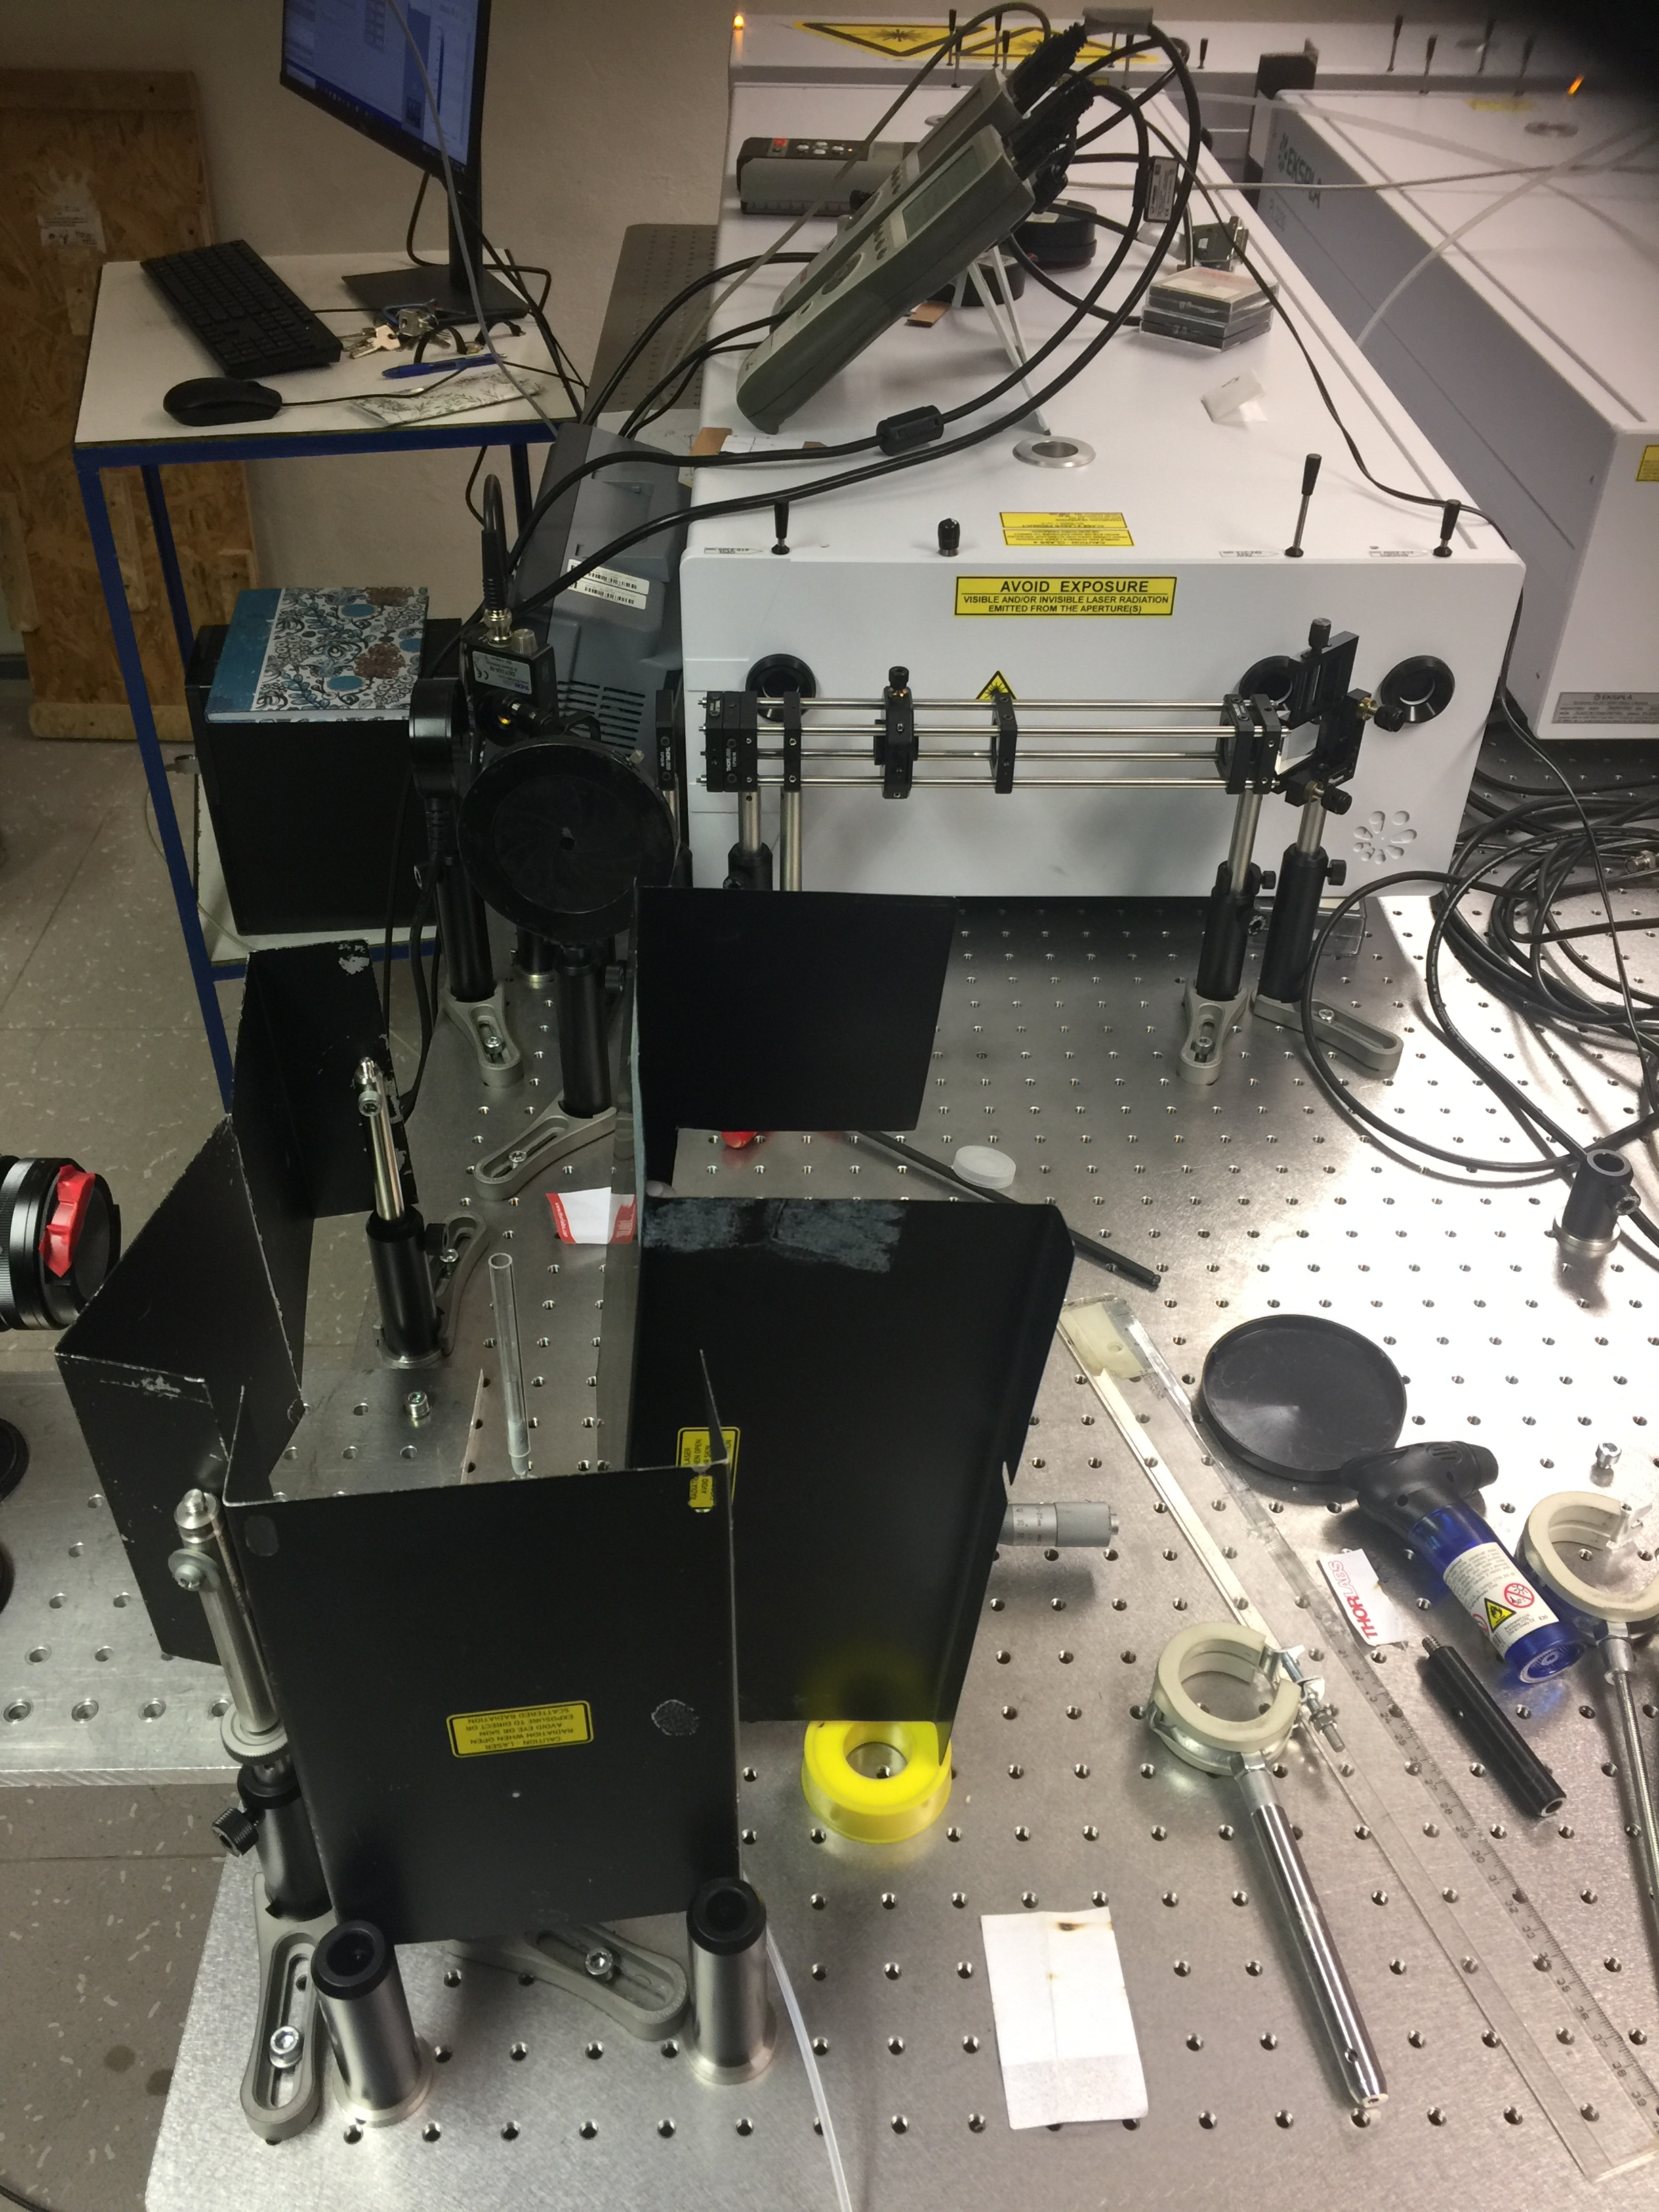
\includegraphics[width=\textwidth, trim={0 24 0 0}, clip]
		{img/lif-setup-photo-1}
	\caption{Snímek sestavené aparatury.
		Laserový svazek vychází druhým otvorem zprava,
		hned za hranolem je rám s~prostorovým filtrem.
		Dělič svazku je zčásti vidět za kruhovou clonou.
		Atomizátor je svislá skleněná trubička.
		Plechové zástěny rozmístěné v~okolí dráhy svazku
		slouží k~odstínění parazitního světla,
		zajištění tmavého pozadí a~k~ochraně plamene před prouděním vzduchu.
		Měřič energie za atomizátorem není vidět, je skryt za nejbližší
		zástěnou.
		Zcela vlevo je vidět objektiv ICCD kamery s~připevněnými
		křemennými sklíčky místo filtru.}%
	\label{fig:lif-setup-photo}
\end{figure}

\section{Vyhodnocení}
\label{sec:lif-method}
Před stanovením koncentrace atomů selenu bylo nutno určit několik
dalších veličin, na nichž výpočet závisí.
Prostřednictvím Rayleighova rozptylu byl zjištěn profil laserového svazku,
který udává prostorové rozložení intenzity excitujícího záření.
Změření excitačního profilu umožnilo nalézt přesnější polohu maxima
fluorescenčního signálu
a~stanovit spektrální překryv laseru a~excitace $\specoverlap$.
Ukázalo se, že fluorescence i~navzdory nízké energii laserových pulzů
projevovala saturaci, kterou bylo tudíž nutno zahrnout do výpočtů.
Podstatným krokem bylo určení doby života zářivého stavu.

Záznam z~ICCD kamery tvoří časová posloupnost jednokanálových sním\-ků,
přičemž každý snímek je tvořen nastaveným počtem akumulací na čipu.
Kamera kromě fluorescence snímá také parazitní signál pocházející
ze zbytkového světla v~laboratoři nebo vlastního záření plamene.
Pro potlačení jejich nežádoucího vlivu
byly všechny snímky korigovány odečtením temného snímku změřeného
s~vypnutým laserem za jinak stejných podmínek a~nastavení.

Pro výpočty byla použita energie laserových pulzů změřená za~atomizátorem.
V~případech, kdy bylo k~dispozici pouze měření za děličem,
byla energie za atomizátorem dopočtena podle závislosti obou energií
v~ostatních měřeních.
% Pro výpočty byla použita energie laserových pulzů změřená za děličem.
Energie byla následně zprůměrována v~časových intervalech odpovídajících
jednotlivým snímkům kamery.
Hranice těchto intervalů byly odhadnuty ze~známé frekvence spouštění
kamery, počtu akumulací na čipu a~vyčítací prodlevy mezi sním\-ky.

Na obrázku č.~\ref{fig:lif-flame} je samotný plamen bez laserové excitace
zaznamenaný ICCD kamerou bez použití filtru.
Intenzita byla v~tomto případě velmi slabá
(plamen byl pouhým okem neviditelný),
snímek je výsledkem \num{10000} akumulací.

\begin{figure}[p]
	\centering
	\input{../lif/results/flame}
	\caption{Snímek plamene bez laseru.
		Kamera byla bez filtru a~nastavena na \num{10000} akumulací.}
	\label{fig:lif-flame}
\end{figure}

\subsection{Profil svazku}
\label{sec:lif-rayleigh}
Pro další vyhodnocení bylo nutno znát skutečný prostorový profil
laserového svazku v~oblasti atomizátoru.
K~jeho zjištění bylo použito slabého rozptylu laserového záření ve vzduchu.
Uspořádání pokusu bylo stejné, jako bylo popsáno výše,
jen atomizátor byl vypnut (neproudil do něj žádný plyn).
Kamera snímala laserový svazek z~boku, zaznamenaný signál byl v~tomto
případě tvořen především Rayleighovým rozptylem svazku na částicích vzduchu.
Příklad takového snímku je na obrázku č.~\ref{fig:lif-beam}.
Snímaná intenzita byla mnohem větší než u~prostého plamene,
uvedený příklad je ze \num{100} akumulací.

\begin{figure}[p]
	\centering
	\input{../lif/results/rayleigh-example}
	\caption{Snímek laserového paprsku ve vzduchu bez plamene.
		Pozorovaný signál je Rayleighův rozptyl.
		Kamera byla bez filtru a~nastavena na \num{100} akumulací.}
	\label{fig:lif-beam}
\end{figure}

\begin{figure}
	\centering
	\input{../lif/results/rayleigh-profile-s}%
	\hfill
	\input{../lif/results/rayleigh-profile-norm-s}
	\caption{Svislý profil laserového svazku pro různé energie pulzu
		určený pomocí Rayleighova rozptylu.
		V~grafu vlevo je změřená intenzita fluorescence sečtená
		ve směru osy $\xpos$.
		Je patrno, že profil je mírně závislý na nastavené energii,
		neboť poloha maximální intenzity se s~rostoucí energií posouvá
		vzhůru (v~grafu doleva).
		Tento posuv je lépe vidět v~pravém grafu, kde jsou profily
		vyhlazené a~normalizované na jedničku.
		Normalizované profily byly použity k~výpočtu svislého
		rozdělení intenzity laserového paprsku pro známé energie pulzu.}
	\label{fig:lif-rayleigh-profile}
\end{figure}

\begin{figure}
	\centerline{\input{../lif/results/rayleigh-time}}
	\caption{Časový vývoj Rayleighova rozptylu v~průběhu jednoho pulzu.
		Signál je integrován v~horizontálním směru (ve směry osy $x$).}
	\label{fig:lif-rayleigh-time}
\end{figure}

\subsection{Excitační profil}
\label{sec:lif-excitprof}
Excitační profil byl změřen postupným laděním laseru na vlnové délky
v~rozsahu \SIrange{195.95}{196.20}{\nano\metre}
s~krokem \SI{0.001}{\nano\metre}.
Pokus byl proveden pro několik energií laserového pulzu $\enlaser$,
jak s~prostorovým filtrem, tak bez něj.

Na základě takto změřeného profilu byla poloha maxima LIF předběžně
odhadnuta na \SI{196.032}{\nano\metre}.
Při dalších měřeních byla vlnová délka laseru na\-stavena na tuto hodnotu.

Naměřená data byla dále aproximována Voigtovým profilem pomocí
Le\-ven\-berg-Marquardtova algoritmu.
Detail proložených profilů pro různé energie pulzu s~prostorovým filtrem
je na obrázku č.~\ref{fig:lif-excitprof-fit}
a~optimalizované parametry jsou v~tabulce č.~\ref{tab:lif-excitprof-fit}.

\begin{figure}
	\centering
	\input{../lif/results/excitprof-nofilter}
	\bigskip\par
	\input{../lif/results/excitprof-filter}
	\caption{Excitační profil bez prostorového filtru (nahoře)
		a~s~prostorovým filtrem (dole) pro několik energií pulzu.}
	\label{fig:lif-excitprof-filter}
\end{figure}

\begin{figure}
	\centering
	\input{../lif/results/excitprof-fit}
	\caption{Detail maxima integrálního excitačního profilu
		změřeného s~prostorovým filtrem
		a~spočtených aproximací Voigtovým profilem.}
	\label{fig:lif-excitprof-fit}
\end{figure}

\shorthandoff{-}
\begin{table}[bh]
	\centering
	\caption{Parametry aproximovaných excitačních profilů.
		$\enlaser$ je energie laserového pulzu,
		$\wavelen_\mathrm{max}$ je střed profilu,
		$\voigtsigma$ a~$\voigtgamma$ jsou šířky Gaussova a~Lorentzova profilu
		a~$\sum\Delta\lif^{2}$ je reziduální suma čtverců.}
	\label{tab:lif-excitprof-fit}
	\sisetup{
		table-alignment-mode = format,
		table-number-alignment = center,
	}
	\pgfplotstabletypeset[
		header = false,
		col sep = tab,
		skip first n = 1,
		every head row/.style = {
			before row = \toprule,
			after row = {
				\midrule
			}
		},
		string type,
		columns = {[index] 0, [index] 1, [index] 2, [index] 3, [index] 4},
		skip rows between index = {0}{5},
		columns/0/.style = {
			column name = $\enlaser\ [\si{\micro\joule}]$,
			column type = {S[
				table-format = 1.2,
				round-mode = places,
				round-precision = 2
			]},
		},
		columns/1/.style = {
			column name = $\wavelen_\mathrm{max}\ [\si{\nano\metre}]$,
			column type = {S[
				table-format = 3.4,
				round-mode = places,
				round-precision = 4
			]},
		},
		columns/2/.style = {
			column name = $\voigtsigma\ [\si{\nano\metre}]$,
			column type = {S[
				table-format = 1.4,
				round-mode = places,
				round-precision = 4
			]},
		},
		columns/3/.style = {
			column name = $\voigtgamma\ [\si{\nano\metre}]$,
			column type = {S[
				table-format = 1.4,
				round-mode = places,
				round-precision = 4
			]},
		},
		columns/4/.style = {
			column name = $\sum\Delta\lif^{2}$,
			column type = {S[
				table-format = 3.2,
				round-mode = places,
				round-precision = 2
			]},
		},
		every last row/.style = {after row = \bottomrule}
	]{../lif/results/excitprof-fit.tsv}
\end{table}
\shorthandon{-}

\subsection{Saturace}
\label{sec:lif-saturation}
Fluorescence podle očekávání vykazovala při použití vyšších intenzit laseru
znám\-ky saturace.
Jelikož tento jev nebyl zanedbatelný, bylo nutno jej vyšetřit,
aby jeho vliv mohl být zohledněn při stanovení koncentrace.

Laserový svazek měl v~místě plamene rovinný nerozbíhavý tvar
o~tloušťce asi \SI{1}{\milli\metre}.
Teoretická závislost LIF v~rovinném svazku při pozorování zboku
byla odvozena v~\cite{lif-pb}, kde je vyjádřena přibližným vztahem:
\begin{equation}
	\label{eq:lif-saturation}
	\lif(\enlasery) = \frac{2\lifslope}{\lifsat}
	\left( 1 - \frac{\ln(1 + \lifsat\enlasery)}{\lifsat\enlasery} \right).
\end{equation}
Zde $\lif$ je intenzita signálu LIF,
$\enlasery$ je intenzita laserového svazku ve výšce $\ypos$
(předpokládá se vodorovné vedení svazku),
a~$\lifslope$, $\lifsat$ jsou neznámé parametry.
Parametr $\lifslope$ popisuje lineární část závislosti pro velmi nízké energie,
parametr $\lifsat$ se nazývá saturační parametr a~udává zakřivení
závislosti v~nasycené oblasti.

Vlnová délka laseru byla držena na konstantní
hodnotě \SI{196.032}{\nano\metre},
zatímco energie pulzu byla postupně nastavována v~rozsahu
od zhruba \SI{0.5}{\micro\joule} do \SI{4.0}{\micro\joule}.

Kvůli rozsahům použitých měřičů bylo nutno měření rozdělit do dvou sérií:
první od \SI{2.0}{\micro\joule} do \SI{4.0}{\micro\joule}
a~druhé od \SI{0.5}{\micro\joule} do \SI{2.0}{\micro\joule}.
Při vyhodnocení se však ukázalo, že data z~obou sérií pro určité místo
ve výboji na sebe nenavazují plynule a~je mezi nimi patrný skok.
Obrázek \ref{fig:lif-saturation-full-example} toto chování ilustruje.
Jako možné vysvětlení se nabízí proměnlivost profilu laserového svazku
při změnách celkové energie pulzu, kterou ani prostorový filtr
nedokázal potlačit úplně.
Tato proměnlivost byla prokázána měřením rozptylu svazku ve~vzduchu,
jak ukazuje obrázek č.~\ref{fig:lif-rayleigh-profile}.

\begin{figure}
	\centering
	\input{../lif/results/saturation-full-example-index}
	\input{../lif/results/saturation-full-example-1}%
	\input{../lif/results/saturation-full-example-2}
	\input{../lif/results/saturation-full-example-3}%
	\input{../lif/results/saturation-full-example-4}
	\caption{Příklad dat z~měření saturace pro několik vybraných bodů.
		Přehledový snímek odpovídá energii pulzu \SI{3.99}{\micro\joule}.
		Níže jsou průběhy signálu $\lif$ v~závislosti na energii
		laseru $\enlaser$.
		Hodnoty $\lif$ v~nižším a~vyšším intervalu energií na sebe
		dobře nenavazují a~je mezi nimi patrný jistý skok,
		který znesnadňuje proložení předpokládanou
		závislostí \eqref{eq:lif-saturation}.
		Tento nesoulad je způsoben změnou svislého rozložení intenzity
		laserového svazku při změně celkové energie pulzu.}
	\label{fig:lif-saturation-full-example}
\end{figure}

Určení prostorově rozlišené saturace z~těchto dat se potýkalo s~obtížemi.
Bylo nutno důkladně zohlednit prostorovou variabilitu intenzity svazku.
Z~měření Rayleighova rozptylu svazku ve vzduchu byly k~dispozici
profily svazku naměřené pro čtyři různé celkové energie pulzu,
tyto profily jsou na obrázku \ref{fig:lif-rayleigh-profile} vlevo.

Profily byly pro odstranění šumu vyhlazeny klouzavým průměrem
a~odečtením pozadí.
Pak byly normovány na hodnotu 1 podle vztahu:
\begin{equation}
	\enlaserynorm = \frac{\enlasery}{\int \enlasery \mathrm{d}y},
\end{equation}
což je vidět na obrázku \ref{fig:lif-rayleigh-profile} vpravo.
Normované profily pro mezilehlé energie byly získány lineární interpolací
mezi naměřenými profily (lineární interpolace zachovává normovanost).
Profil intenzity v~každém snímku byl spočten vynásobením příslušného
normovaného profilu celkovou energií pulzu.
Výsledný průběh intenzit je na obrázku
č.~\ref{fig:lif-saturation-full-profile}.

\begin{figure}[htp]
	\centering
	\input{../lif/results/saturation-full-profile}
	\caption{Profil laserového svazku pro různé energie pulzu,
		integrovaný ve směru osy $\xpos$.
		Červené křivky jsou naměřené profily,
		modré křivky byly interpolovány z~naměřených.
		Každá interpolovaná křivka přísluší jednomu snímku kamery.
		Je zřetelný posuv maxima intenzity k~nižším hodnotám $\ypos$
		s~rostoucí energií.}
	\label{fig:lif-saturation-full-profile}
\end{figure}

Závislost intenzity fluorescence $\lif$ na energii laseru $\enlaser$
byla aproximována funkcí \eqref{eq:lif-saturation} pomocí metody
nejmenších čtverců, čímž byly získány parametry $\lifslope$ a~$\lifsat$.
Toto vyhodnocení bylo provedeno zvlášť pro každý pixel snímku,
přičemž každý snímek byl za účelem potlačení šumu vyhlazen klouzavým
průměrem ve čtverci o~rozměru \num{5}\times\SI{5}\pixel.

Spočtené hodnoty intenzitního parametru $\lifslope$ a~saturačního
parametru $\lifsat$ jsou na obrázku~\ref{fig:lif-saturation-full-params}
spolu s~ukázkou aproximovaných průběhů.
Je vidět, že parametr $\lifslope$ je soustředěn do centrální oblasti
nad atomizátorem, zatímco jinde jsou jeho hodnoty velmi nízké.
Za povšimnutí stojí, že směrem vzhůru roste, navzdory předpokladu,
že bude výraznější v~nižší části plamene.

Saturační parametr $\lifsat$ vykazuje při aproximaci větší nestabilitu
a~jeho hodnoty i~rozložení výrazně závisely na provedené korekci profilu
intenzity svazku $\enlasery$.
Na obrázku je jeho hodnota v~oblasti plamene zhruba homogenní:
Je sice patrn nárůst s~rostoucí výškou, stejně jako u~parametru $\lifslope$,
ale ve vodorovném směru se jeví stabilní.

\begin{figure}
	\centering
	\small
	\input{../lif/results/saturation-full-paramsfits}
	\caption{Parametry fluorescence $\lifslope$ a~$\lifsat$
		určené z~korigovaných hodnot energie
		a~příklad aproximovaných závislostí pro několik pixelů.
		Pro potlačení šumu byly snímky z~kamery před zpracováním vyhlazeny
		průměrováním ve čtverci o~rozměrech \num{5}\times\SI{5}{\pixel}.
		Je patrno, že saturační parametr $\lifsat$ je
		v~oblasti plamene ve vodorovném směru přibližně homogenní.}
	\label{fig:lif-saturation-full-params}
\end{figure}

Je nutno zdůraznit silnou závislost vypočteného saturačního parametru
na předpokládaném profilu laserového svazku.
Obrázek \ref{fig:lif-saturation-full-params-bad} ukazuje extrémní případ,
kdy byla k~vyhodnocení použita vždy jen jedna sada měření ze dvou.
První sada používala vyšší energie pulzu a~intenzita svazku byla soustředěna
více nahoře, druhá sada se pohybovala v~nízkých energiích
(zhruba do \SI{2}{\micro\joule}) a~největší intenzita svazku se nacházela níže.
Jak je z~obrázků patrno, výsledky se zásadně liší.
U~parametru $\lifslope$ je zachována vodorovná homogenita,
ale výškové rozdělení je zcela jiné.
U~saturačního parametru $\lifsat$ jakákoli rovnoměrnost zcela vymizela.

\begin{figure}[htp]
	\centering
	\small
	\input{../lif/results/saturation-full-params-bad}
	\caption{Ukázka nevhodného vyhodnocení parametrů $\lifslope$ a~$\lifsat$
		jako důkaz toho, že výsledky jsou velice citlivé na korekci intenzit.
		Nahoře jsou parametry spočítané z~datové sady vyšších energií,
		dole ze~sady nižších energií, kde je intenzita laseru soustředěna níže.
		Je vidět, že uvažovaný profil laserového svazku má značný vliv
		na výsledky.
		Zatímco parametr $\lifslope$ zůstává alespoň ve vodorovném směru
		homogenní, o~parametru $\lifsat$ nelze nic takového říci.
		Posun maxima intenzity směrem vzhůru navíc silně nadhodnocuje
		horní část snímané oblasti oproti dolní (viz grafy nahoře).}
	\label{fig:lif-saturation-full-params-bad}
\end{figure}

Alternativou k~výše uvedenému postupu je svislé rozlišení vůbec neuvažovat
a~obě veličiny, to jest intenzitu fluorescence $\lif$ i~intenzitu
laseru $\enlasery$, integrovat ve směry $\ypos$.
(V~případě intenzity laserového svazku to znamená vzít přímo
naměřenou hodnoty energie pulzu $\enlaser$.)
Obdobný postup, jako byl popsán výše, pak vede na vodorovně rozlišené
parametry $\lifslope$ a~$\lifsat$ na obrázku~\ref{fig:lif-saturation-x-params}.

\begin{figure}[htp]
	\centering
	\small
	\input{../lif/results/saturation-x-params}
	\caption{Parametry $\lifslope$ a~$\lifsat$ spočtené z~dat integrovaných
		ve směru svislé osy $\ypos$.
		Vodorovná čára označuje hodnotu $\lifsat$ spočítanou z~integrální
		intenzity celého snímku.
		Svislé čáry označují polohu ukázkových průběhů v~dolním obrázku.}
	\label{fig:lif-saturation-x-params}
	\bigskip
	\input{../lif/results/saturation-x-fits}
	\caption{Naměřená data pro vybrané polohy $\xpos$ a~spočtené proklady.
		Data v~nižším a~vyšším rozsahu energií na sebe dobře navazují,
		protože svislá proměnlivost profilu laserového svazku je skryta
		použitím celkové energie pulzu $\enlaser$.}
	\label{fig:lif-saturation-x-fits}
\end{figure}

\subsection{Doba života}
\label{sec:lif-lifetime}
Druhým významným ukazatelem koncentrace částic je doba života $\lifetime$,
tedy parametr exponenciálního poklesu signálu v~čase.
Časový vývoj fluorescence byl zaznamenán opakovaným měřením mnoha pulzů
s~postupně zvyšovaným zpožděním kamery za laserovým pulzem.
Délka každé expozice byla nastavena na \SI{2}{\nano\second},
po provedení 100 akumulací bylo vždy zpoždění kamery zvýšeno
o~\SI{0.5}{\nano\second}.
Takto byl zaznamenán časový interval o~délce \SI{30}{\nano\second}.
Atomizátor byl přitom nastaven na obvyklý průtok.

Série snímků na obrázku č.~\ref{fig:lif-timeev} ukazuje výběr několika
snímků z~tohoto měření.
Je vidět, že pulz, který dorazí zhruba v~čase $\SI{5}{\nano\second}$,
způsobí velmi rychlý nárůst fluorescence, která dosáhne maxima kolem
času $\SI{7}{\nano\second}$ a~poté výrazně pomaleji slábne.
Tímto poklesem intenzity byla proložena exponenciální funkce,
jejíž konstanta $\lifetime$ z~exponentu je doba života.

Spočtená doba života pro každý pixel středové oblasti snímku je
na obrázku \ref{fig:lif-lifetime-full-params}.
Je patrno, že ve~středu plamene je doba života nejvyšší
a~směrem k~okrajům slábne.
Vně plamene je signál velmi slabý a~spočtené hodnoty $\lifetime$
nejsou věrohodné.

Náročnost zpracování byla v~tomto případě výrazně nižší než u~saturace,
neboť doba života nezávisí na absolutní velikosti signálu
a~nebylo proto nutné provádět korekci na proměnlivost profilu
laserového svazku.
Ukázka prokládaných dat pro několik pixelů je
na obrázku~\ref{fig:lif-lifetime-full-params} dole.

\begin{figure}[p]
	\centering
	\input{../lif/results/timeev}
	\caption{Typický vývoj fluorescenčního signálu v~průběhu jedné periody.
		Časové rozlišení bylo získáno opakovaným měřením mnoha period
		s~postupnou změnou zpoždění kamery za začátkem pulzu.
		Pulz začíná přibližně v~čase $\tim = \SI{5.0}{\nano\second}$.
		Kamera byla ve všech snímcích nastavena na \num{100} akumulací.
		Hloubka snímané oblasti, daná tloušťkou laserového svazku,
		je zhruba \SI{1}{\milli\metre}.}
	\label{fig:lif-timeev}
\end{figure}

\begin{figure}[htp]
	\centering
	\input{../lif/results/lifetime-full-params}
	\input{../lif/results/lifetime-full-fits}
	\caption{Určená doba života $\lifetime$.
		Body po stranách obrázku jsou spočítané z~velmi malých hodnot
		signálu a~nejsou proto věrohodné.
		Níže je příklad proložených dat pro několik vybraných bodů.}
	\label{fig:lif-lifetime-full-params}
\end{figure}

Protože doba života v~plném rozlišení je značně zatížena šumem,
byla kromě ní spočtena i~doba života ze svisle integrovaných dat,
obdobně jako v~případě saturace.
Tato vodorovně rozlišená doba života je vykreslena
na obrázku~\ref{fig:lif-lifetime-x-params}.
Zde je jasně zřetelné, že její maximum leží zhruba ve středu plamene
a~směrem ke krajům klesá.
Pozoruhodné je, že závislost se zdá být velmi podobná lineární.
Ukázka prokladů ve vybraných bodech je
na obrázku~\ref{fig:lif-lifetime-x-fits}.
Zde je patrno, že svislá integrace signálu měla za následek potlačení šumu
a~tím pádem přesnější proklady.

\begin{figure}[htp]
	\centering
	\input{../lif/results/lifetime-x-params}
	\caption{Doba života $\lifetime$ určená z~dat integrovaných ve směru
		svislé osy $\ypos$.
		Barevné čáry označují polohu ukázkových průběhů níže.}
	\label{fig:lif-lifetime-x-params}
	\bigskip
	\input{../lif/results/lifetime-x-fits}
	\caption{Naměřená data integrovaná ve směry $\ypos$ a~proložený
		exponenciální pokles pro vybrané polohy $\xpos$.}
	\label{fig:lif-lifetime-x-fits}
\end{figure}

\section{Výsledky}
\label{sec:lif-results}

\begin{figure}[htp]
	\centering
	\input{../lif/results/concentration-single}
	\caption{Koncentrace atomů selenu určená z~jednoho snímku.}
	\label{fig:lif-concentration-single}
\end{figure}
